\section{Actividades y Metodología}

%Localización física y ubicación de instalaciones:

El proyecto se llevará a cabo en la Facultad de Ingeniería de la Universidad Nacional de La Plata.
Los ensayos necesarios se realizarán en el Área Técnica de Electrónica e Instrumental (ATEI)
del Departamento de Electrotecnia de la Facultad de Ingeniería de la UNLP.
Se realizarán consultas semanales con el tutor para el seguimiento del desarrollo del proyecto y
la revisión de decisiones tomadas por el equipo de trabajo.

Para alcanzar las metas y los objetivos propuestos, se realizarán las siguientes actividades:

\subsection{Estudio de bibliografía y diseño}
Con el objetivo de capacitarse, se estudiarán y analizarán aspectos de seguridad, curvas de carga de la batería 
y topologías de conversores de potencia, de acuerdo con los requerimientos del proyecto. 
Se evaluarán las diferentes alternativas posibles y, en base a su complejidad y a su costo,
se elegirá la solución más adecuada para el logro de los objetivos. 

Se realizarán simulaciones en SPICE (programa de simulación con énfasis en circuitos integrados),
separando el proceso en 4 partes:
\begin{itemize}
    \item Fuente conmutada: Convierte la tensión alterna de la red doméstica en una tensión continua.
    \item Fuente de corriente: Brinda una corriente constante a la batería durante la primera etapa de carga.
    \item Circuito de control: Alterna entre las etapas de carga.
    \item Circuito de protección: Protege a la batería en caso de cortocircuito.
\end{itemize}

En la Figura \ref{fig:esquema_cargador} se puede observar un esquema en bloques del cargador.
De izquierda a derecha, los primeros dos bloques representan el circuito de la fuente conmutada,
seguidos por el bloque de la fuente de corriente en la parte superior y debajo de este se encuentra el bloque de control.
El circuito de protección está integrado en los bloques de control y fuente de corriente.

%incluir esquema de cargador
\begin{figure}
    \centering
    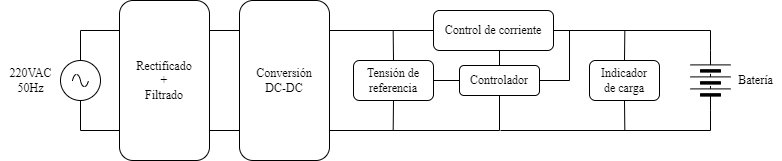
\includegraphics[width=\textwidth]{images/esquema_cargador.png}
    \caption{Esquema del cargador}
    \label{fig:esquema_cargador}
\end{figure}

Se realizará un análisis crítico de las primeras simulaciones y, en base a los resultados obtenidos, 
se corregirán los circuitos propuestos. 
Esta etapa finaliza con el diseño de un circuito impreso y la presentación del informe parcial. 

\subsection{Implementación}
Se construirá un prototipo funcional que cumpla con las especificaciones propuestas. 
Debido a que el costo de una batería de litio de las características necesarias es elevado,
se evaluará la posibilidad de realizarlo a escala con una batería de menor tensión y/o capacidad.

\subsection{Validación}
Una vez terminado el proceso de diseño e implementación,
se verificará que el prototipo cumpla con las especificaciones presentadas.